\documentclass[12pt,twoside]{article}

%---------------------------------%
%__Inclusions de packages__%
%_Packages Basiques_%
  \usepackage[utf8x]{inputenc}
  \usepackage[T1]{fontenc}
  \usepackage[francais]{babel}
  \usepackage{textcomp}

  \usepackage{schemabloc}
  \usepackage{hyperref}
  
  \usepackage{bigcenter}

  \usepackage{verbatim} %Environnement pour Ècrire du code \begin{verbatimtab}[10] pour 10 espaces par tabulation
  \usepackage{moreverb}

%Inclure Images
  \usepackage{graphicx} % Pour l'ajout d'images (commande \includegraphics[height=200, width=600]{chemin})
  
%Placer les floats
  \usepackage{placeins} %\FloatBarrier pour placer 

%Maths
  \usepackage{amsmath} % Pour fraction complexes
  \usepackage{amssymb} %math
  \usepackage{mathrsfs} %math
  \usepackage{siunitx} % Notation complexe : \num{}

%Pour les figures
  \usepackage{wrapfig}
  \usepackage{tikz}
  \usepackage{float}


%---------------------------------%
%__Quelques configurations__%
%_Annexes_%
  \usepackage{appendix}\renewcommand{\appendixtocname}{Annexes} 		\renewcommand{\appendixpagename}{Annexes} 

%_Présentation et marges_%
  \usepackage{layout}
  \usepackage[top=2cm, bottom=3cm, left=2cm, right=2cm]{geometry} %Marges
  \pagestyle{plain} %Plain : Seulement numero en bas de page, sinon mettre headings
  \marginparwidth = 0.mm

%_LstListings_%
  %Package
    \usepackage{listings} %Environnement pour écrire du code
	\usepackage{xcolor}
	\usepackage{times}
  
  %Config Langage VHDL
    \lstset{
    language=VHDL,
    basicstyle=\ttfamily\small,
    breaklines=true,
    prebreak=\raisebox{0ex}[0ex][0ex]{\ensuremath{\hookleftarrow}},
    frame=lines,
    showtabs=false,
    showspaces=false,
    showstringspaces=false,
    keywordstyle=\color{red}\bfseries,
    stringstyle=\color{green!50!black},
    commentstyle=\color{gray}\itshape,
    numbers=left,
    captionpos=t,
    escapeinside={\%*}{*)}
	}
    
%_Commandes rapides pour maths_%
\renewcommand{\deg}{\ensuremath{^\circ}}

%---------------------------------%
%__Informations pour le document__%
  \title{\textsc{\textbf{Projet S8}} - IMA4\\~\\
  \Large{\textit{\bsc{Rapport} - Décodage de codeurs en quadrature de phase sur FPGA}}
  }
  \date{}
  \author{
   Benjamin \bsc{Lafit}\and
   Valentin \bsc{vergez}
   }

%---------------------------------%
%__Début du document__%
\begin{document}

%_Première page
	% Titre du document	
	\maketitle

	% Table des matières
	\renewcommand{\contentsname}{Table des matières}
	\tableofcontents % Table des matières
	\newpage
	
	% Images	
%	\FloatBarrier
%	\newpage
%
%	\begin{figure}[h!]
%  		\centering
%  		%\includegraphics[width=0.7\textwidth]{img/crbIBoucleCourantAvecFiltre0_7}
% 		\caption{Boucle de courant - Réponse indicielle (80A), avec filtre, $\zeta = 0.7$}
%  		\label{img:crbBoucleCourantAvecFiltre0_7}
%	\end{figure}	
%	\FloatBarrier ~
	
	%% CDC ETENDU Wiki	
%Cahier des charges étendu
%
%Description
%Ce projet s'inscrit dans le cadre de la réalisation d'un robot mobile autonome, capable de se déplacer avec précision grâce au retour de ses capteurs. La propulsion du robot est effectuée par deux moteurs à courant-continu, chacun couplé à une roue motrice tandis que le retour sur le déplacement est lui obtenu par deux codeurs à quadratures de phases couplés à des roues de mesures. Il est aussi possible de récupérer l'information de vitesse des moteurs grâce à des dynamos tachymétriques ou par le biais d'autres codeurs à quadratures de phases directement couplés au moteur.
%Pour approcher ce fonctionnement, on travaillera initialement sur un seul codeur et un seul moteur. L'objectif est d'interpréter les signaux en quadratures de phases avec un FPGA et d'effectuer à partir de cette information un asservissement en vitesse du moteur.
%Si ce fonctionnement de base est obtenu suffisamment tôt, des améliorations sont envisageables, comme par exemple :
%Commande et mesure pour plusieurs moteurs et codeurs ;
%Pilotage du FPGA par un protocole de communication (série, CAN, I2C, à déterminer …) ;
%Asservissement polaire (cas d'un déplacement de robot) ;
%Calcul d'odométrie.
%La liste est non exhaustive.
%Travail à réaliser 
%FPGA :
%Récupération des signaux codeurs ;
%Interprétation des signaux et comptage ;
%Écriture de la mesure sur un bus ;
%Lecture de la consigne d'asservissement ;
%Asservissement et génération de la consigne moteur.
%Électronique de puissance :
%Carte de conversion consigne (signaux logiques) en commande (tension avec puissance) ;
%Éventuelle protection en tension et en courant de la carte.
%Caractéristiques 
%Les moteurs utilisés peuvent être de deux types différents :
%Graupner Speed 720 BB Torque.
%Alimenté en 0-12V avec des courants max de 3A et des courants moyens de 750mA.
%Faulhaber 3557K024CS.
%Alimenté en 0-24V avec des courants max de 1,1A et des courants moyens de 65mA.
%Ces deux types de moteurs représentent des cas très usités, il conviendra donc d'avoir une carte de puissance permettant d'assumer ces deux configurations.
	
%_Inclusion du contenu
	\FloatBarrier
	\section{Introduction}
% Introduction a proprement parler
En robotique mobile mais aussi plus largement dans beaucoup de domaines techniques, il est souvent nécessaire d'obtenir des informations sur des distances parcourues.
\\Dans l'industrie, ça peut concerner par exemple l'avance d'un tapis roulant ou encore la rotation d'un plateau tournant.
\\En robotique mobile plus  spécifiquement, un robot doit se repérer dans l'espace et savoir effectuer des déplacements précis. Pour ce faire, une méthode simple est de récupérer les informations de distance sur le déplacement puis de les traiter.\\

Pour faire ces mesures, il existent plusieurs catégories de capteurs.\\
Celle qui nous intéresse est celle des encodeurs et plus spécifiquement les encodeurs à signaux en quadratures de phases.\\
Un encodeur est un dispositif qui va retransmettre un mouvement ou une position sous la forme d'un codage particulier.\\

Le principe de codage à signaux en quadratures de phases sera détaillé plus tard.\\

% Problématique
\subsection{Problématique}
Notre projet s'inscrit dans le cadre du club Robotech Lille, club de robotique de l'école Polytech Lille, et de la Coupe de France de Robotique organisée par Planètes Sciences.\\

Cette Coupe de Robotique exige la conception et la réalisation de robots mobiles autonomes.\\
A Robotech Lille, les informations propre au déplacement sont données par ces fameux encodeurs à signaux à quadratures de phases.\\
Il est donc nécessaire que soit intégrée au robot un système de décodage des signaux à quadratures de phase.\\

Précédemment, le robot était géré par un unique micro-contrôleur, aussi en charge du décodage de ces signaux.\\
Cette année est née la volonté d'attribuer la gestion complète du déplacement du robot à un sous-module, facilement réutilisable et indépendant de la structure du robot. Il a été décidé, pour des raisons que nous allons voir ensuite, que ce sous-module allait \^etre géré par un FPGA\footnote{Field-Programmable Gate Array, un réseau de portes programmables (Voir 
\href{http://fr.wikipedia.org/wiki/Circuit_logique_programmable}{Wikipedia : Circuits Programmables})}. La gestion du décodage des signaux en quadrature de phase doit donc \^etre elle aussi assumée par le FPGA, c'est à cette partie là que nous nous intéressons.\\

% Etat de l'art
\newpage
\subsection{\'Etat de l'art}
Le principe de base des encodeurs à signaux en quadrature de phases est de générer deux signaux carrés identiques, décalées de $\pm90\deg$. Ce décalage contient une information importante, il permet de savoir si le codeur rotatif tourner dans le sens trigonométrique ou anti-trigonométrique.\\

Ces signaux carrés proviennent en fait de deux capteurs qui signale le passage ou non d'un marquage placé sur un disque tournant avec le rotor du codeur. \\ Si le disque ne contient d'un marquage, une période du signal indiquera que le codeur a effectué un tour complet.\\
L'encodeur que nous utilisons possède lui 1024 marques sur son disque, on dit alors que le codeur a une résolution de 1024 ticks par tours.\\

Pour interpréter ces ticks et ce décalage puis les traduire en une position, en un comptage/décomptage, on utilise traditionnellement des circuits logiques intégré dédiés à cela. On peut aussi utiliser un micro-contrôleur pour effectuer cette t\^ache, seulement si le codeur tourne vite, à raison de plusieurs milliers de ticks par tours, les fréquences des signaux à interpréter deviennent importantes et trop encombrantes pour le micro-contrôleur.\\
L'inconvénient des circuit intégrés est leur difficulté d'intégration. Pour une utilisation ponctuelle, leur volume est trop important au regard de leur fonction et il est parfois difficile de les interfacer au reste de l'application (gros bus de données). Parfois ils sont intégrés aux micro-contrôleurs, le problème devient alors leur nombre limité ou le prix.\\
La solution FPGA se présente comme un intermédiaire très intéressant. Le principe de fonctionnement du FPGA permet de retrouver les performances identiques aux circuits intégrés (puisqu'il s'agit simplement d'intégrer le fonctionnement de ces circuits dans le FPGA). Il permet aussi d'obtenir un système beaucoup plus complet, comme celui qu'assumerait un micro-contrôleur, mais avec une fiabilité et une robustesse inégalable.\\
L'inconvénient est l'aspect statique de l'application et la difficulté d'implémentation, c'est d'ailleurs pour cette raison qu'il est rare de trouver des systèmes de déplacement complet gérés ainsi.\\

% Contenu du document
\newpage
\subsection{Contenu du projet}
Le sujet initial propose de réaliser un système simple sur cible FPGA permettant de :
\begin{itemize}
\item Lire et décoder des signaux en quadrature de phase en provenance d'une ou plusieurs roues codeuses ;
\item Asservir un ou plusieurs moteurs, soit pas-à-pas soit à courant continu.
\end{itemize}

La cible visée est un FPGA de chez Xilinx (carte de développement LX9 à base de Spartan 3\footnote{Le Spartan 3 est un modèle de FPGA de la marque Xilinx}).\\
En parallèle, une carte d'interface de puissance doit \^etre réalisée, c'est l'interface entre FPGA et moteurs.\\

Les objectifs du sujet sont atteints. Dans ce document sera expliqué le principe du décodage de signaux utilisé, l'asservissement, la génération de signaux logique de commande du moteur, la carte de puissance d'interfaçage FPGA - Moteur ainsi qu'un élément supplémentaire.\\
En effet, comme la finalité de ce projet est d'être utilisé dans un sous-module complet, nous avons commencé à implémenter une interface série avec une mémoire interne au FPGA. L'objectif est d'avoir un module fonctionnel, complètement configurable et pilotable par liaison série. Ainsi, les utilisateurs futures n'auront qu'à effectuer les branchements du module à leur robot et à le commander avec leurs autres modules électroniques, via liaison série. Ils n'auront pas à se soucier du fonctionnement interne, il s'agira d'une boîte noire.\\

Toutefois, comme ce sous-module peut-être sujet à des améliorations, les codes sources sont bien sûr fournis aux utilisateurs et doivent permettre une mise à jour facile de l'application.\\
C'est en tout cas pour ce soucis d'utilisation facile que nous avons choisis ce système de pilotage série.\\



	% NB : Include créer des nouvelles pages pour inclure le contenu
	% Input inclus le contenu directement dans le texte
	
	% Decodage
		% Principe

		% Adaptation de tensions		
		
		% Problème de rebonds
		
	% Asservissement
		% Principe
	\begin{center}
	\begin{tikzpicture}
	\sbEntree{E}
	\sbComp{comp}{E}                 
	\sbRelier[$E_1$]{E}{comp}
	\sbBloc{reg}{Régulateur}{comp}   
	\sbRelier[$\epsilon$]{comp}{reg}
	\sbBloc{pwm}{PWM}{reg}         
	\sbRelier[C]{reg}{pwm}    
	\sbBloc{sys}{Système}{pwm}       
	\sbRelier[U]{pwm}{sys}
	\sbSortie{S}{sys}                
	\sbRelier[$S_1$]{sys}{S}
	\sbDecaleNoeudy[4]{S}{U}
	\sbBlocr{cap}{Mesure (QuadDecoder)}{U}        
	\sbRelieryx{sys-S}{cap}
	\sbRelierxy[m]{cap}{comp}
	\end{tikzpicture}
	\end{center}
		
		% Numérique
		
		% Asservissement polaire
			% Principe
		
	% Interface série
	\FloatBarrier
	\section{Interface série}
Dans le but d'établir une communication entre le Raspberry (partie intelligente) et le FPGA nous avons adopter un mode de communication série. Ce protocole étant relativement simple à 
coder et à mettre en place, c'est pourquoi nous avons décider de l'utiliser au sein du robot pour l'échange de données.

\subsection{Reception}
Ce programme agit sur chaque front montant de l'horloge. Son but sera de permettre la réception des
données à 9600 bauds(debit paramétrable par une variable générique).
A chaque front montant de l'horloge,nous incrémentons un compteur
de 1 jusqu'à compter la période d'un bit (5208 dans le cas d'une transmission à 9600 bauds avec un horloge de 50MHz). Lorsque ce chiffre est atteint nous récupérons la
valeur du bit Rx et la stockons dans la variable data\_next par décalage à chaque fois. De cette
manière nous aurons, dans data\_next, la valeur des bits du message mais dans le sens inverse. A
chaque récupération de bit, la variable i est incrémentée de afin de connaître la fin de réception de
la donnée.
Au premier front d'horloge (bit de start à 1), le compteur est initialisé à sa moitié afin que la
récupération des données se fasse au milieu de la période du bit pour être sur d'avoir la bonne
valeur.
Lorsque i=nombre bit de données + 2 (le nombre de bit de données est paramétrable par une variable générique), tous les bits du messages ont été enregistrés.
Nous écrivons donc la donnée ainsi reçue sur le registre de sortie de manière inversée (oData(0)=Data\_next(8) ...).

\subsection{Emission}
Ce programme, sur chaque front montant va commencer la transmission si le bit iEnableTransmit est à l'état haud. A ce moment là on va incrémenter un compteur qui
permettra de faire une communication à un debit donné. C'est à dire que pour une communication à 9600 baud par exemple, on doit laisser le bit de data à son état 
pendant 5208 coups d'horloge avec un horloge à 50MHz. De plus, ce module établie une communication série avec un bit de start (passage de 1 à 0), un nombre de bit de donné
paramétrable (doit être le même en emission et réception) et un bit de stop.
On avons donc une communication très simple, sans détection/correction d'erreurs.

\subsection{Module de gestion}
Le module de gestion permettra d'instancier les deux composants précédemment créés et de faire un mappage complet des entrées sorties. Ainsi nous n'aurons plus qu'un module
général où toutes les entrées sorties seront déclarées. De même, c'est dans ce fichier où il suffira de changer les différents paramètres génériques pour configurer la communication
(fréquence d'horloge, débit de communication, nombre de bit de données).

	
	% PWM
	\FloatBarrier
	\section{Interface PWM}
Le module de PWM permet de contrôler un moteur grâce à une modulation par largeur d'impulsion(Pulse Width Modulation). Ce module prends en entrée un valeur sur 8bits permettant de régler la valeur
du rapport cyclique de la PWM.

Afin de créer un signal PWM, il a fallu coder un programme qui incrémente un compteur tout les cycles d'horloge puis met la sortie à l'état haut tant que le compteur est 
inféreur à la valeur du rapport cyclique. Lorsque le compteur dépasse la valeur du rapport cyclique, la sortie passe à l'état bas jusqu'à ce que le compteur arrive à 255. A ce
moment là, le compteur repasse à 0 et on recommence.

Ci dessous, une image d'une PWM avec un rapport cyclique de 33\%, la valeur en entrée est de 77.

\begin{figure}[h]
\centering
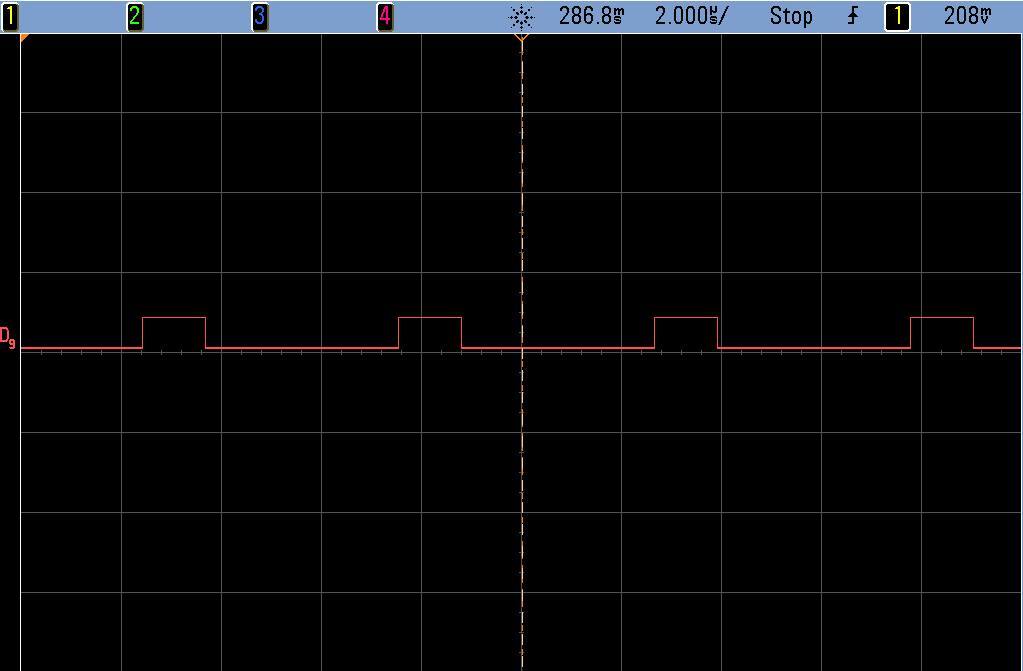
\includegraphics[width=10cm]{img/PWM_3F.png}
\caption{Exemple de signal PWM}
\end{figure}
\pagebreak
	
	% Carte de puissance
	\FloatBarrier
	\section{Carte de puissance}
Partie décrivant le fonctionnement de la carte de puissance
	
	\FloatBarrier
	% Ameliorations possibles
%\section{Améliorations possibles}

% Conclusion à proprement parler
\section{Conclusion}
Ce projet nous a permis de mettre en oeuvre nos connaissances en automatique et en FPGA. Nous avons pu approndir la programmation en langage VHDL, chose que
nous n'étudions que peu en IMA.  
Ce projet n'est pour le moment pas finalisé puisque des améliorations sont à venir, en vu d'une implantation dans le robot concourant dans la coupe de France de robotique
2014. 
	
	\FloatBarrier
	% Annexes
	\appendix
	\appendixpage
	\addappheadtotoc

\lstinputlisting[caption={QuadDecoder.vhd}]{../../src/QuadDecoder.vhd}
\lstinputlisting[caption={Reception série},firstline=20]{../../../Serial/src/serial_rx.vhd}
\lstinputlisting[caption={Emission série},firstline=20]{../../../Serial/src/serial_tx.vhd}
\lstinputlisting[caption={Module gestion de la communication série complète},firstline=20]{../../../Serial/src/serial_module.vhd}
%	\begin{tikzpicture}
%	\sbEntree{E}
%	\sbComp{a}{E}
%	\sbBloc{b}{$H_1$}{a}
%	          \sbRelier[$E_1$]{E}{a}
%	\sbBlocL{c}{$H_2$}{b}
%	          \sbRelier[$\epsilon$]{a}{b}
%	\sbComph{d}{c}
%	          \sbRelier[u]{c}{d}
%	\sbBlocL{e}{$H_3$}{d}
%	\sbBlocL{f}{$H_4$}{e}
%	\sbSortie[5]{S1}{f}
%	          \sbRelier{f}{S1}
%	          \sbNomLien[0.8]{S1}{$S_1$}
%	\sbDecaleNoeudy[-4]{f}{u}
%	\sbDecaleNoeudy{e}{v}
%	\sbBlocr{r1}{$R_1$}{u}
%	\sbBlocr{r2}{$R_2$}{v}
%	\sbBlocrL{r3}{$R_3$}{r2}
%	\sbRelieryx{f-S1}{r1}
%	\sbRelierxy[n1]{r1}{d}
%	\sbRelieryx{e-f}{r2}
%	\sbRelierxy[n2]{r3}{a}
%	\end{tikzpicture}


\end{document}